\chapter{Riemann Pump Circuit design - Implementation of the Riemann Pump approach}
In fact of the high energy consumption, the realized DAC is designed for the integration in a base station. Because it converts a digital bit sequence into an analog rf signal it is implemented in the transmitting path. Based on the idea of a push-pull stage the load impedance of the charge pump is designed first.
\section{Calculation of the load impedance}
Based on the idea to design  a DAC for the transmitting path of a base station, a pre-power amplifier is taken to calculate the load impedance. The first assumption is that the load is a pre-power amplifier which generate a power of \SI{20}{\watt}. To generate this power, the gate periphery of a GaN25 HEMT has to be \SI{4}{\milli \metre} based on the approximation(- official reference???) \SI[per-mode=fraction]{5}{\watt\per\milli\metre}. To get this gate periphery four transistor in parallel each with 8 finger and \SI{125}{\micro \metre} are designed for the power amplifier. The bias point is determined with the MAG. Therefore the following load impedance could be determined.
\begin{equation}
Z = R - jX_c
\end{equation}

In the smith chart Fig. \ref{fig:smith_load_impedance} it is shown that the input impedance of the load is capacitive. The real part of the impedance is roughly $R = \SI{1.89}{\ohm}$, while the imaginary part is capacitive. An important point is the input capacitance is increasing with frequency. While it is normal that the imaginary part of the impedance is increasing with frequency, the input capacitance is not.

 \begin{figure}[ht]
	\centering
  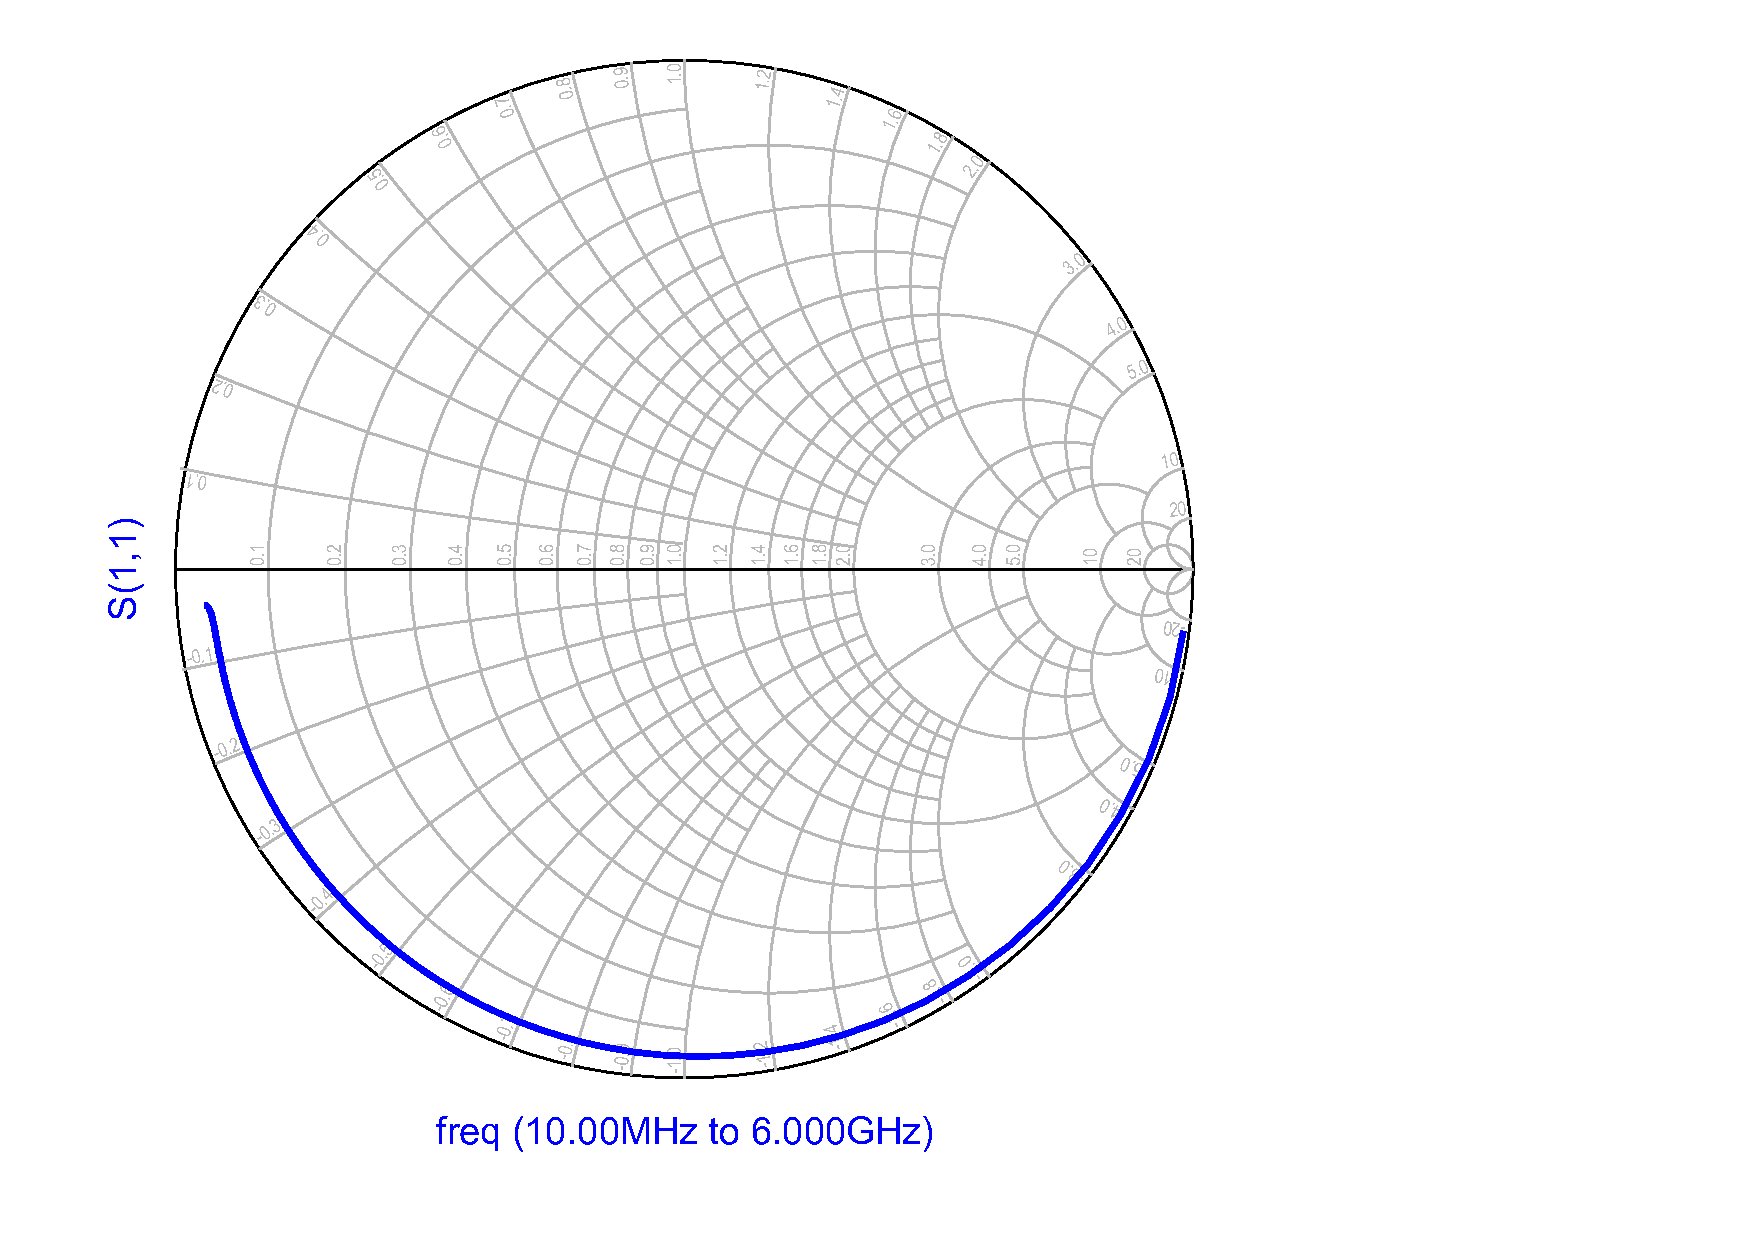
\includegraphics[width=1\textwidth]{S_param_LoadImpedance.pdf}
	\caption{smith chart representing the load impedance}
	\label{fig:smith_load_impedance}
\end{figure}

The input capacitance is calculated through the impedance with:
\begin{equation}
imag[Z_{in}] = X_c
\end{equation}

\begin{equation}
imag[Z_{in}] = \frac{1}{\omega C}
\end{equation}

\begin{equation}
imag[Z_{in}] = \frac{1}{2 \pi f C}
\end{equation}

\begin{equation}
C = \frac{1}{2 \pi f imag[Z_{in}]}
\end{equation}

 \begin{figure}[ht]
	\centering
  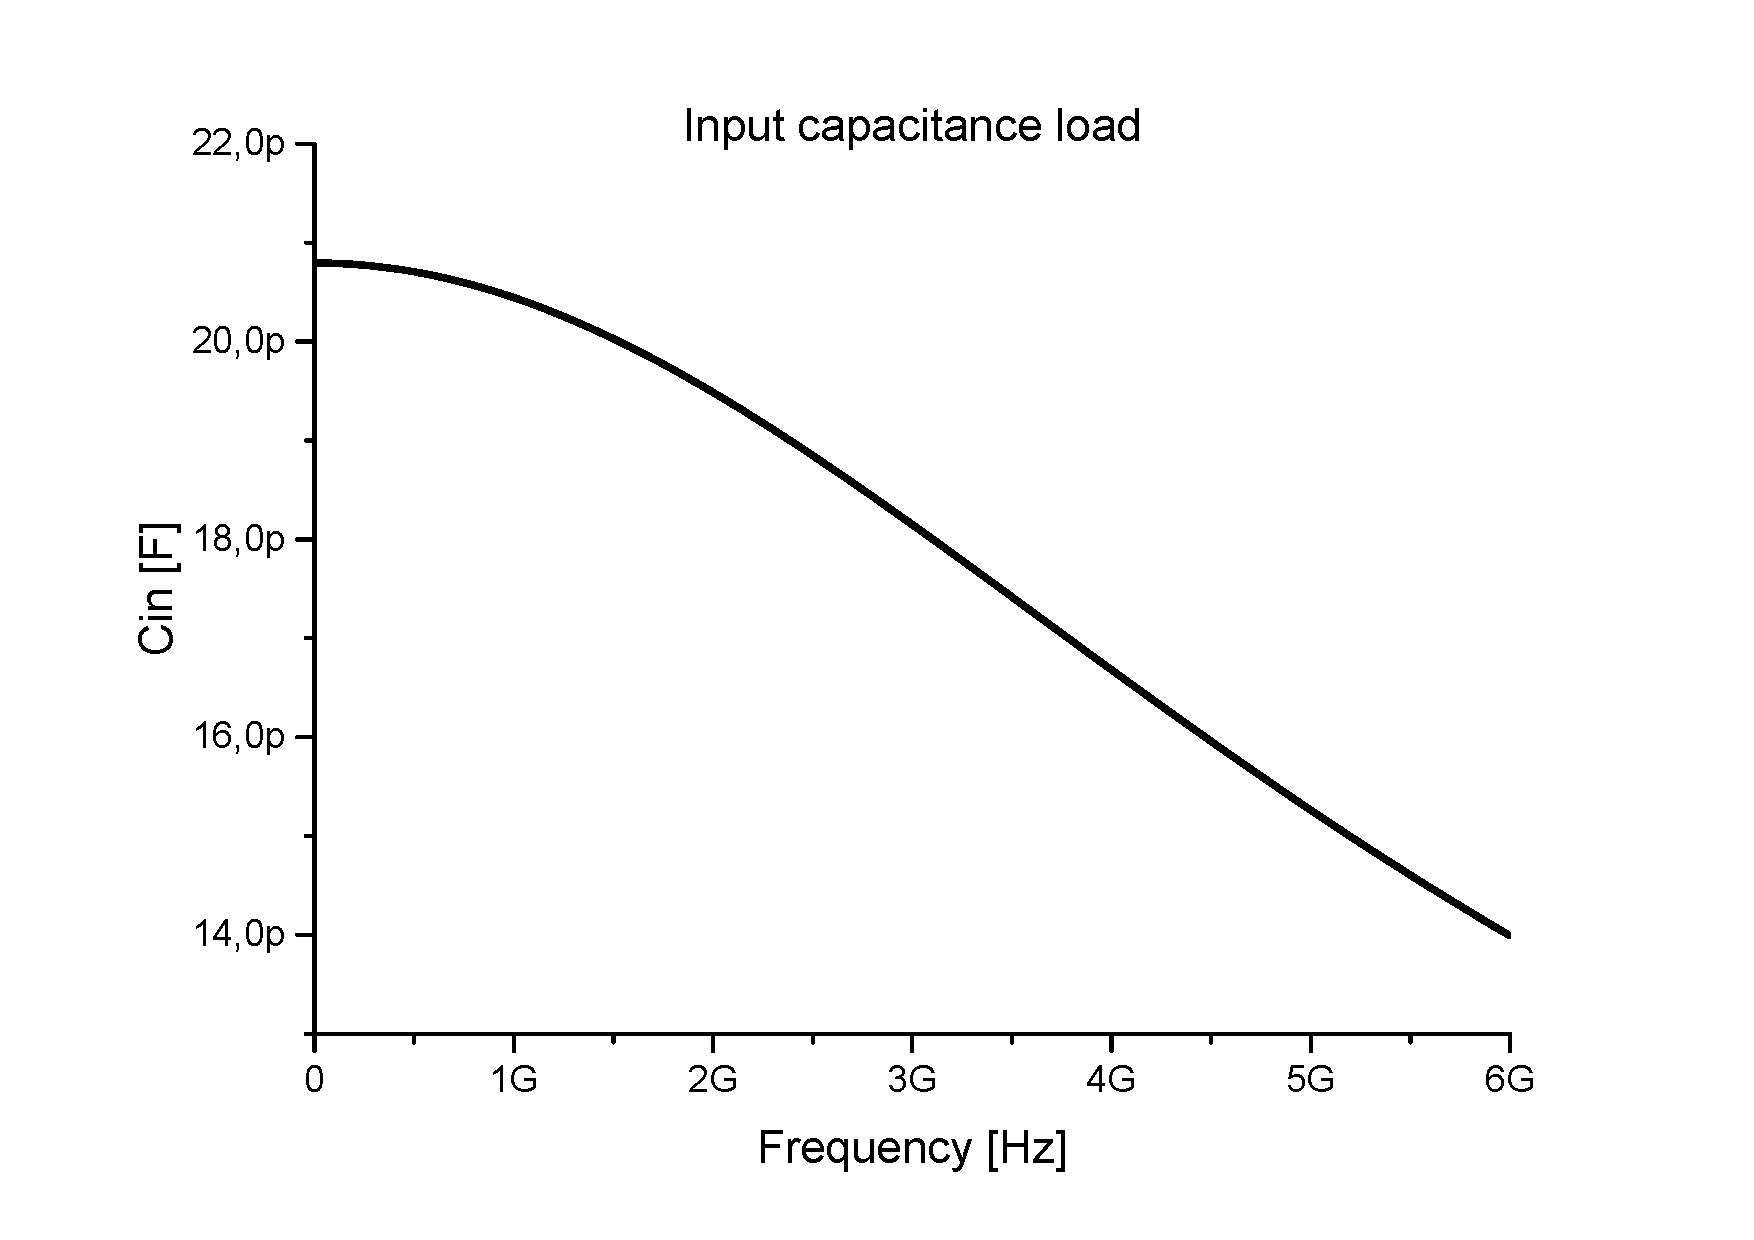
\includegraphics[width=0.5\textwidth]{InputCap_LoadImpedance_6GHz.pdf}
	\caption{frequency dependent input capacitance of the load}
	\label{fig:smith_load_impedance}
\end{figure}
\section{Dimension of the used components}
The transistor dimension were... Different for driver circuit and power circuit... resistor to reduce the energy  consumption, for higher efficiency. \\ The
approach of the push-pull stage Maksimovic, Maroldt.\\
Approach of theoretical and synthesized signal -> MatLab generation of Riemanncode, SNR.\\ Stability, driver concept, energy consumption, frequency bandwidth, gain
Schematic design in Advanced Design System 2014. concept, ideas... 
\textbf{length of the bonds, number of bonds, thickness of bonds ask Dirk Meder. A lot of vias - more inductance - voltage drop between layers. short as possible lines, no rechtecke - para caps in the edge. first filter cap to supply pin near the chip. number and cap size determined on experience. }\\
Control voltage of 5 V realization with OPAMPS? Possible to overdrive opamps instead of using broadband ppa. 

\section{Implementation of the Riemann Pump}
The concept of the Riemann Pump as seen in Fig. \ref{fig:RiemannPumpConcept} is realised with the design tool ADS.

\begin{figure}[ht]
	\centering
  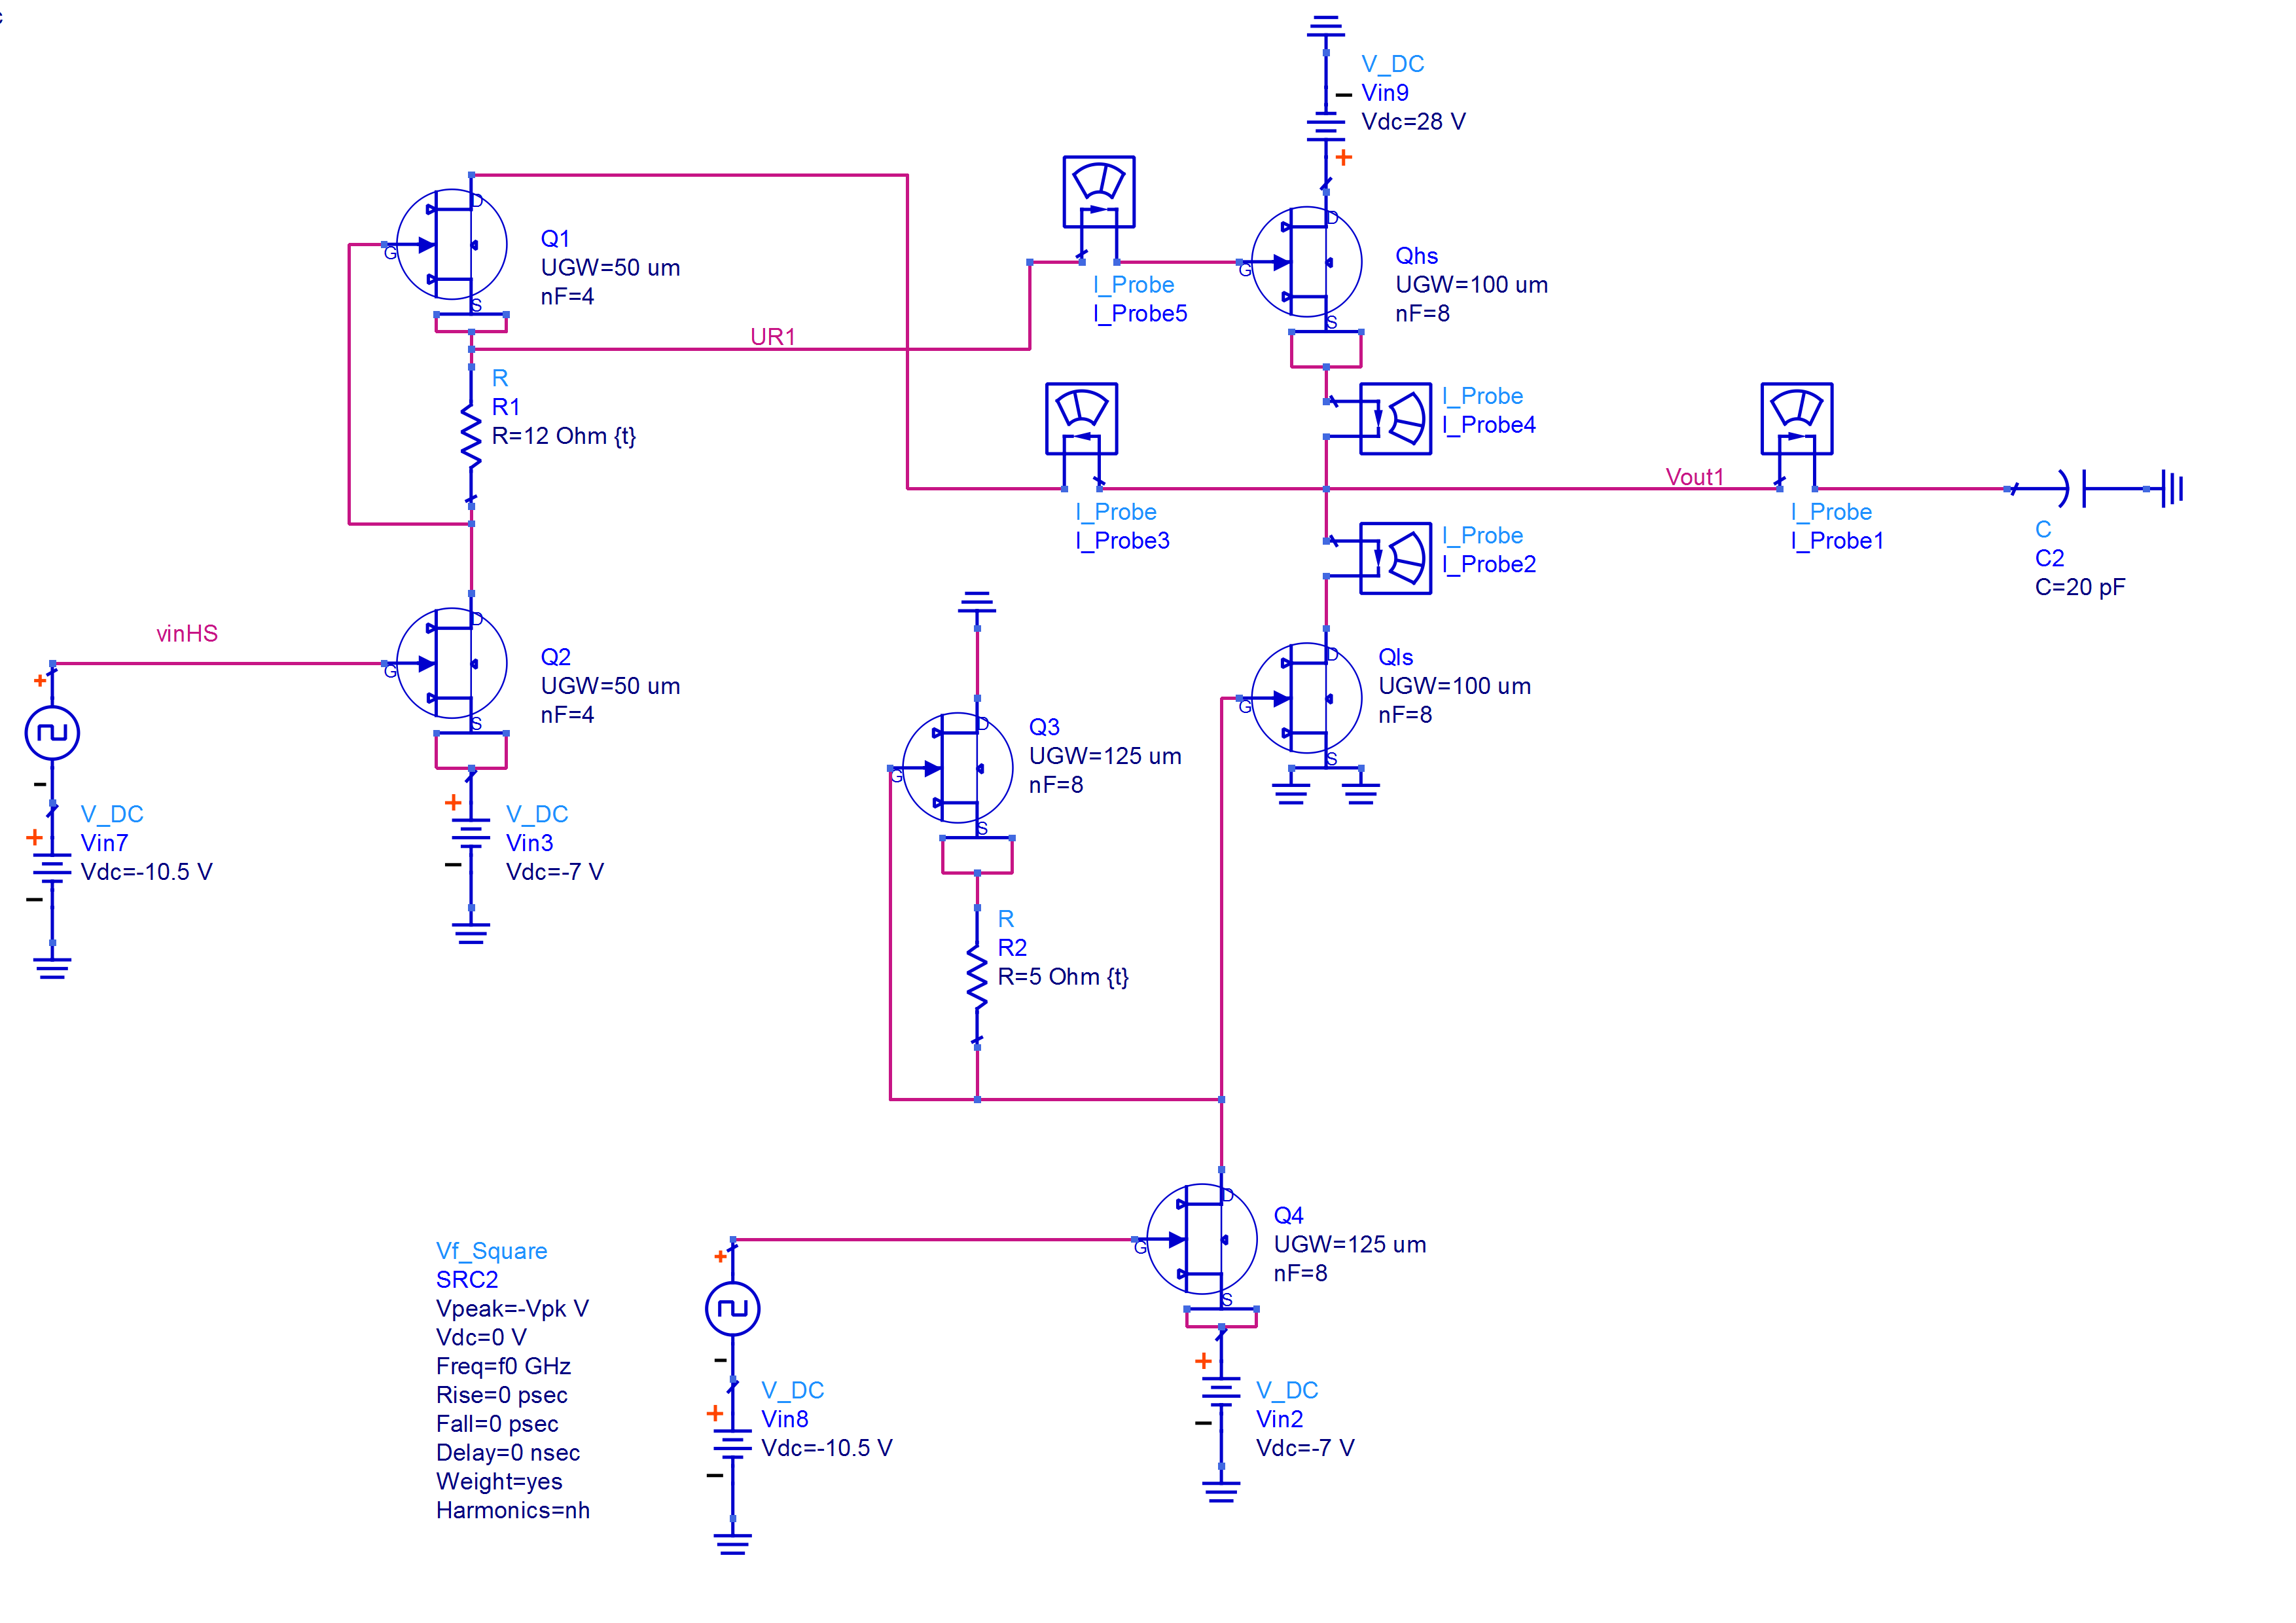
\includegraphics[width=1\textwidth]{Active_PullUp3.png}
	\caption{Schematic of a driver circuit with push-pull stage representing one bit of the DAC called Riemann Pump}
	\label{RiemannPump}
\end{figure}